\section*{Revisjonshistorie}
\begin{center}
 \begin{tabular}{|p{2.5cm} p{5.5cm}|} 
 \hline
 År & Forfatter \\ [0.5ex] 
 \hline\hline
 2020 & Kolbjørn Austeng\\
 \hline
 2021 & Kiet Tuan Hoang\\
 \hline
 2022 & Kiet Tuan Hoang \\ 
 \hline
 2023 & Kiet Tuan Hoang \\
      & Tord Natlandsmyr \\
 \hline
 2024 & Terje Haugland Jacobsson \\
      & Tord Natlandsmyr \\
 \hline
\end{tabular}
\end{center}

\begin{alphasection}
\section{Introduksjon - Kort om Nordic nRF52 DK}
Nordic nRF52 Development Kit er et utviklingskort (se figur \ref{fig:nrf52dk}) utviklet av Nordic Semicoductor i Trondheim. Vi skal på denne laben bruke utviklingskortet til å utforske programvareutvikling med mikrokontrollere.

\begin{figure}[H]
    \centering
    \begin{subfigure}{0.5\textwidth}
    \centering
        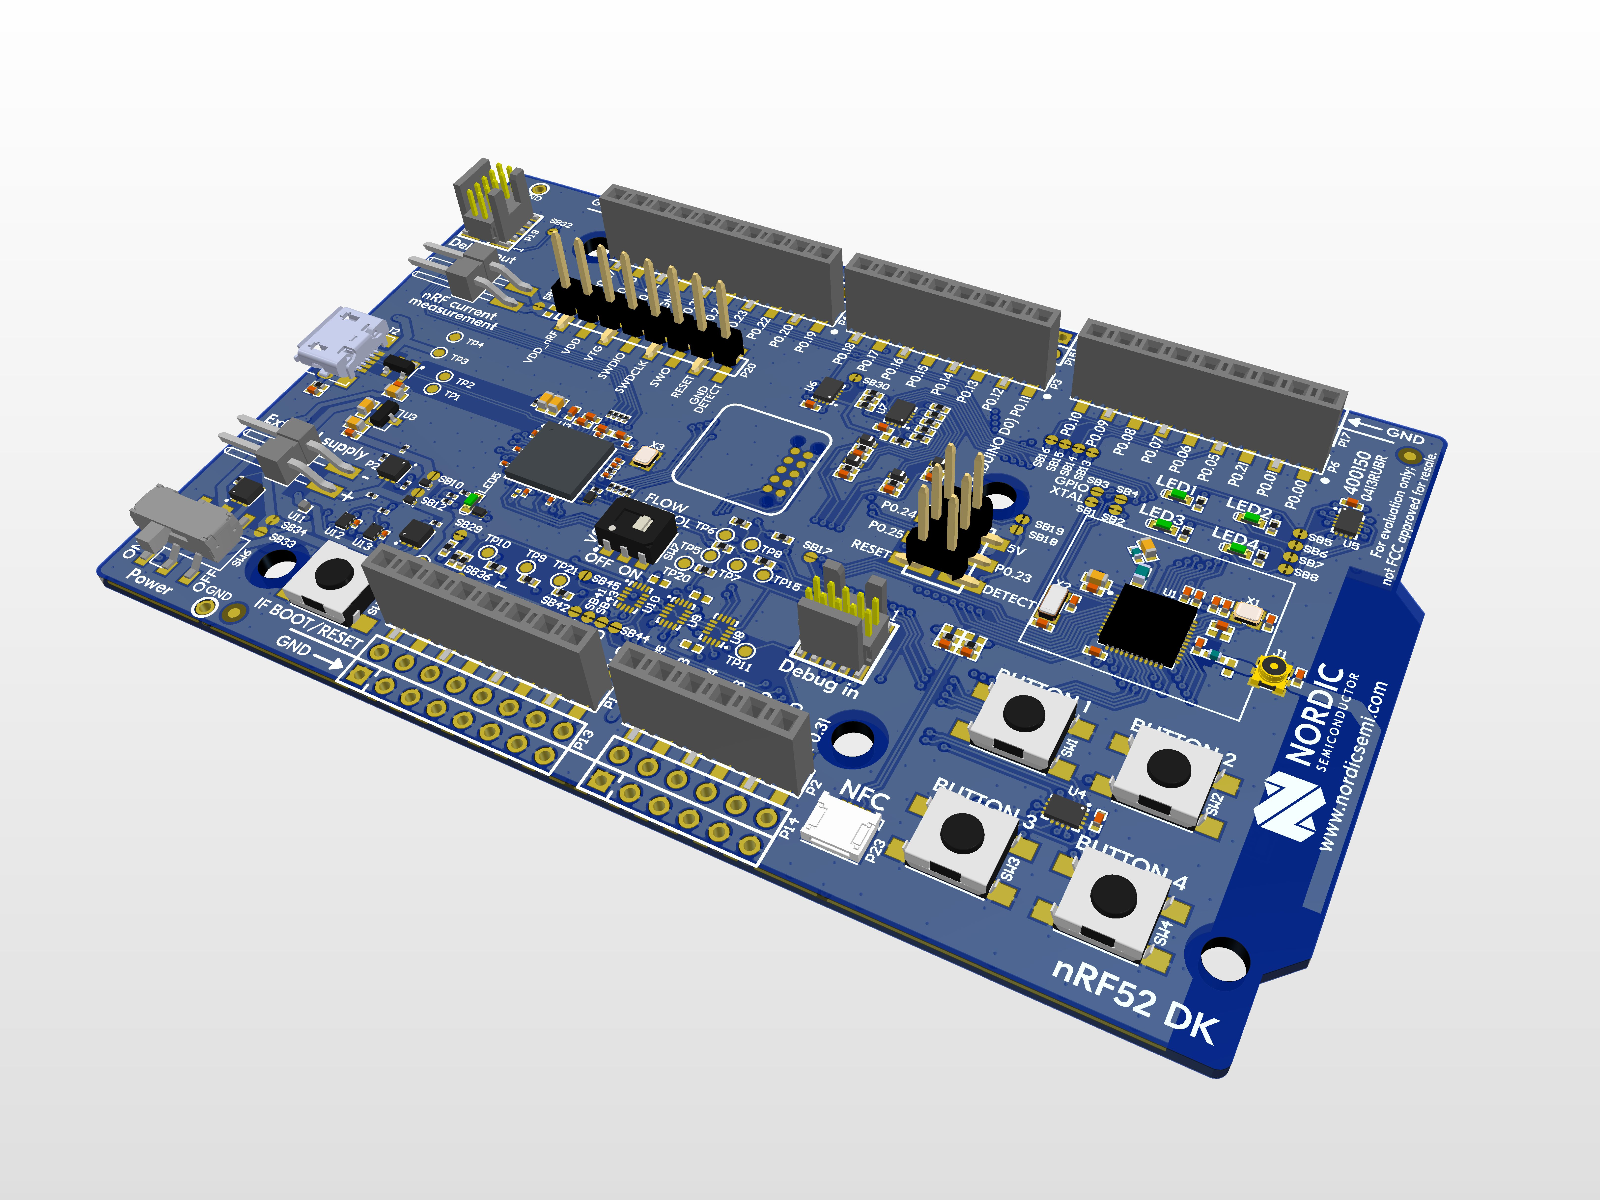
\includegraphics[width=.8\linewidth]{figures/nrf52dk_3d_render.png}
        \caption{3D Render}
    \end{subfigure}%
    \begin{subfigure}{0.5\textwidth}
    \centering
        \includegraphics[width=0.8\linewidth]{figures/nrf52dk.png}
        \caption{Forsiden med led-lys og knapper}
    \end{subfigure}
    \caption{Nordic nRF52 DK brukt i mikrokontrollerlaben.}
    \label{fig:nrf52dk}
\end{figure}


Utviklingskortet er utstyrt med en Arm Cortex-M4 prosessor med en klokkefrekvens på 64 MHz, 512/256 kB flash og  64 kB RAM. Det er ingen hemmelighet at tilpassede datasystemer har blitt utrolig kraftig. En smart USB-C-lader i dag er omtrent 500 ganger raskere enn Apollo 11 sitt navigasjonssystem \footnote{Utregnet av Forrest Heller \href{https://forrestheller.com/Apollo-11-Computer-vs-USB-C-chargers.html}{i denne artikkelen her}}. Utviklingskitet vi jobber med i denne laben har støtte for å kjøre et lite operativsystem, men for å få mest mulig om mikrokontrollere holder vi oss på et maskinnært abstraksjonslag, ofte kalt "bare-metal". Vi snakker ofte om abstraksjonslag i programvareutvikling. Enkelt forklart er hensikten med abstraksjonslag å forenkle noe ved å skjule unødvendige detaljer. Dette impliserer at å gå ned i abstraksjonslag vil introdusere kompleksitet. Dette vil dere få oppleve i denne laben. Funksjoner som kun trenger én linje kode på operativsystemnivå (f.eks. \verb|Print()| i Python) vil kreve betydelig mer kode på en mikrokontroller. Fordelen med et lavere abstraksjonslag er at man har mer kontroll over hva prosessoren faktisk gjør. 

I denne laben vil vi utforske hvordan de forskjellige abstraksjonslagene henger sammen ved å programmere mikrokontrollerens registre direkte. Dette gjøres i \verb|C|, som er det laveste abstraksjonsnivået vi har tilgang til, uten å gå over til ARM-prosessorens instruksjonssett.

Hvis du ser nøye etter på utviklingskitet, vil du legge merke til at den har to chipper: en større merket med N5340, og en mindre merket med N52832. Den har nemlig to mikrokontrollere, også kalt {MCU}-er (\textbf{M}icro\textbf{c}ontroller \textbf{U}nit): En som kjører programvare utelukkende for å programmere og feilsøke hovedchippen, og en som faktisk kjører koden vår. Vi skiller mellom dem med ved navnene "Target" og "Interface". Når du kobler til utviklingskitet til en datamaskin, vil datamaskinen kommunisere med interface MCU-en og oppdage den som USB-lagringsenhet. Interface MCU-en på nRF52 DK kjører SEGGER J-Link Onboard. Den brukes til å programmere og feilsøke Target MCU.


\begin{figure}[H]
    \centering
    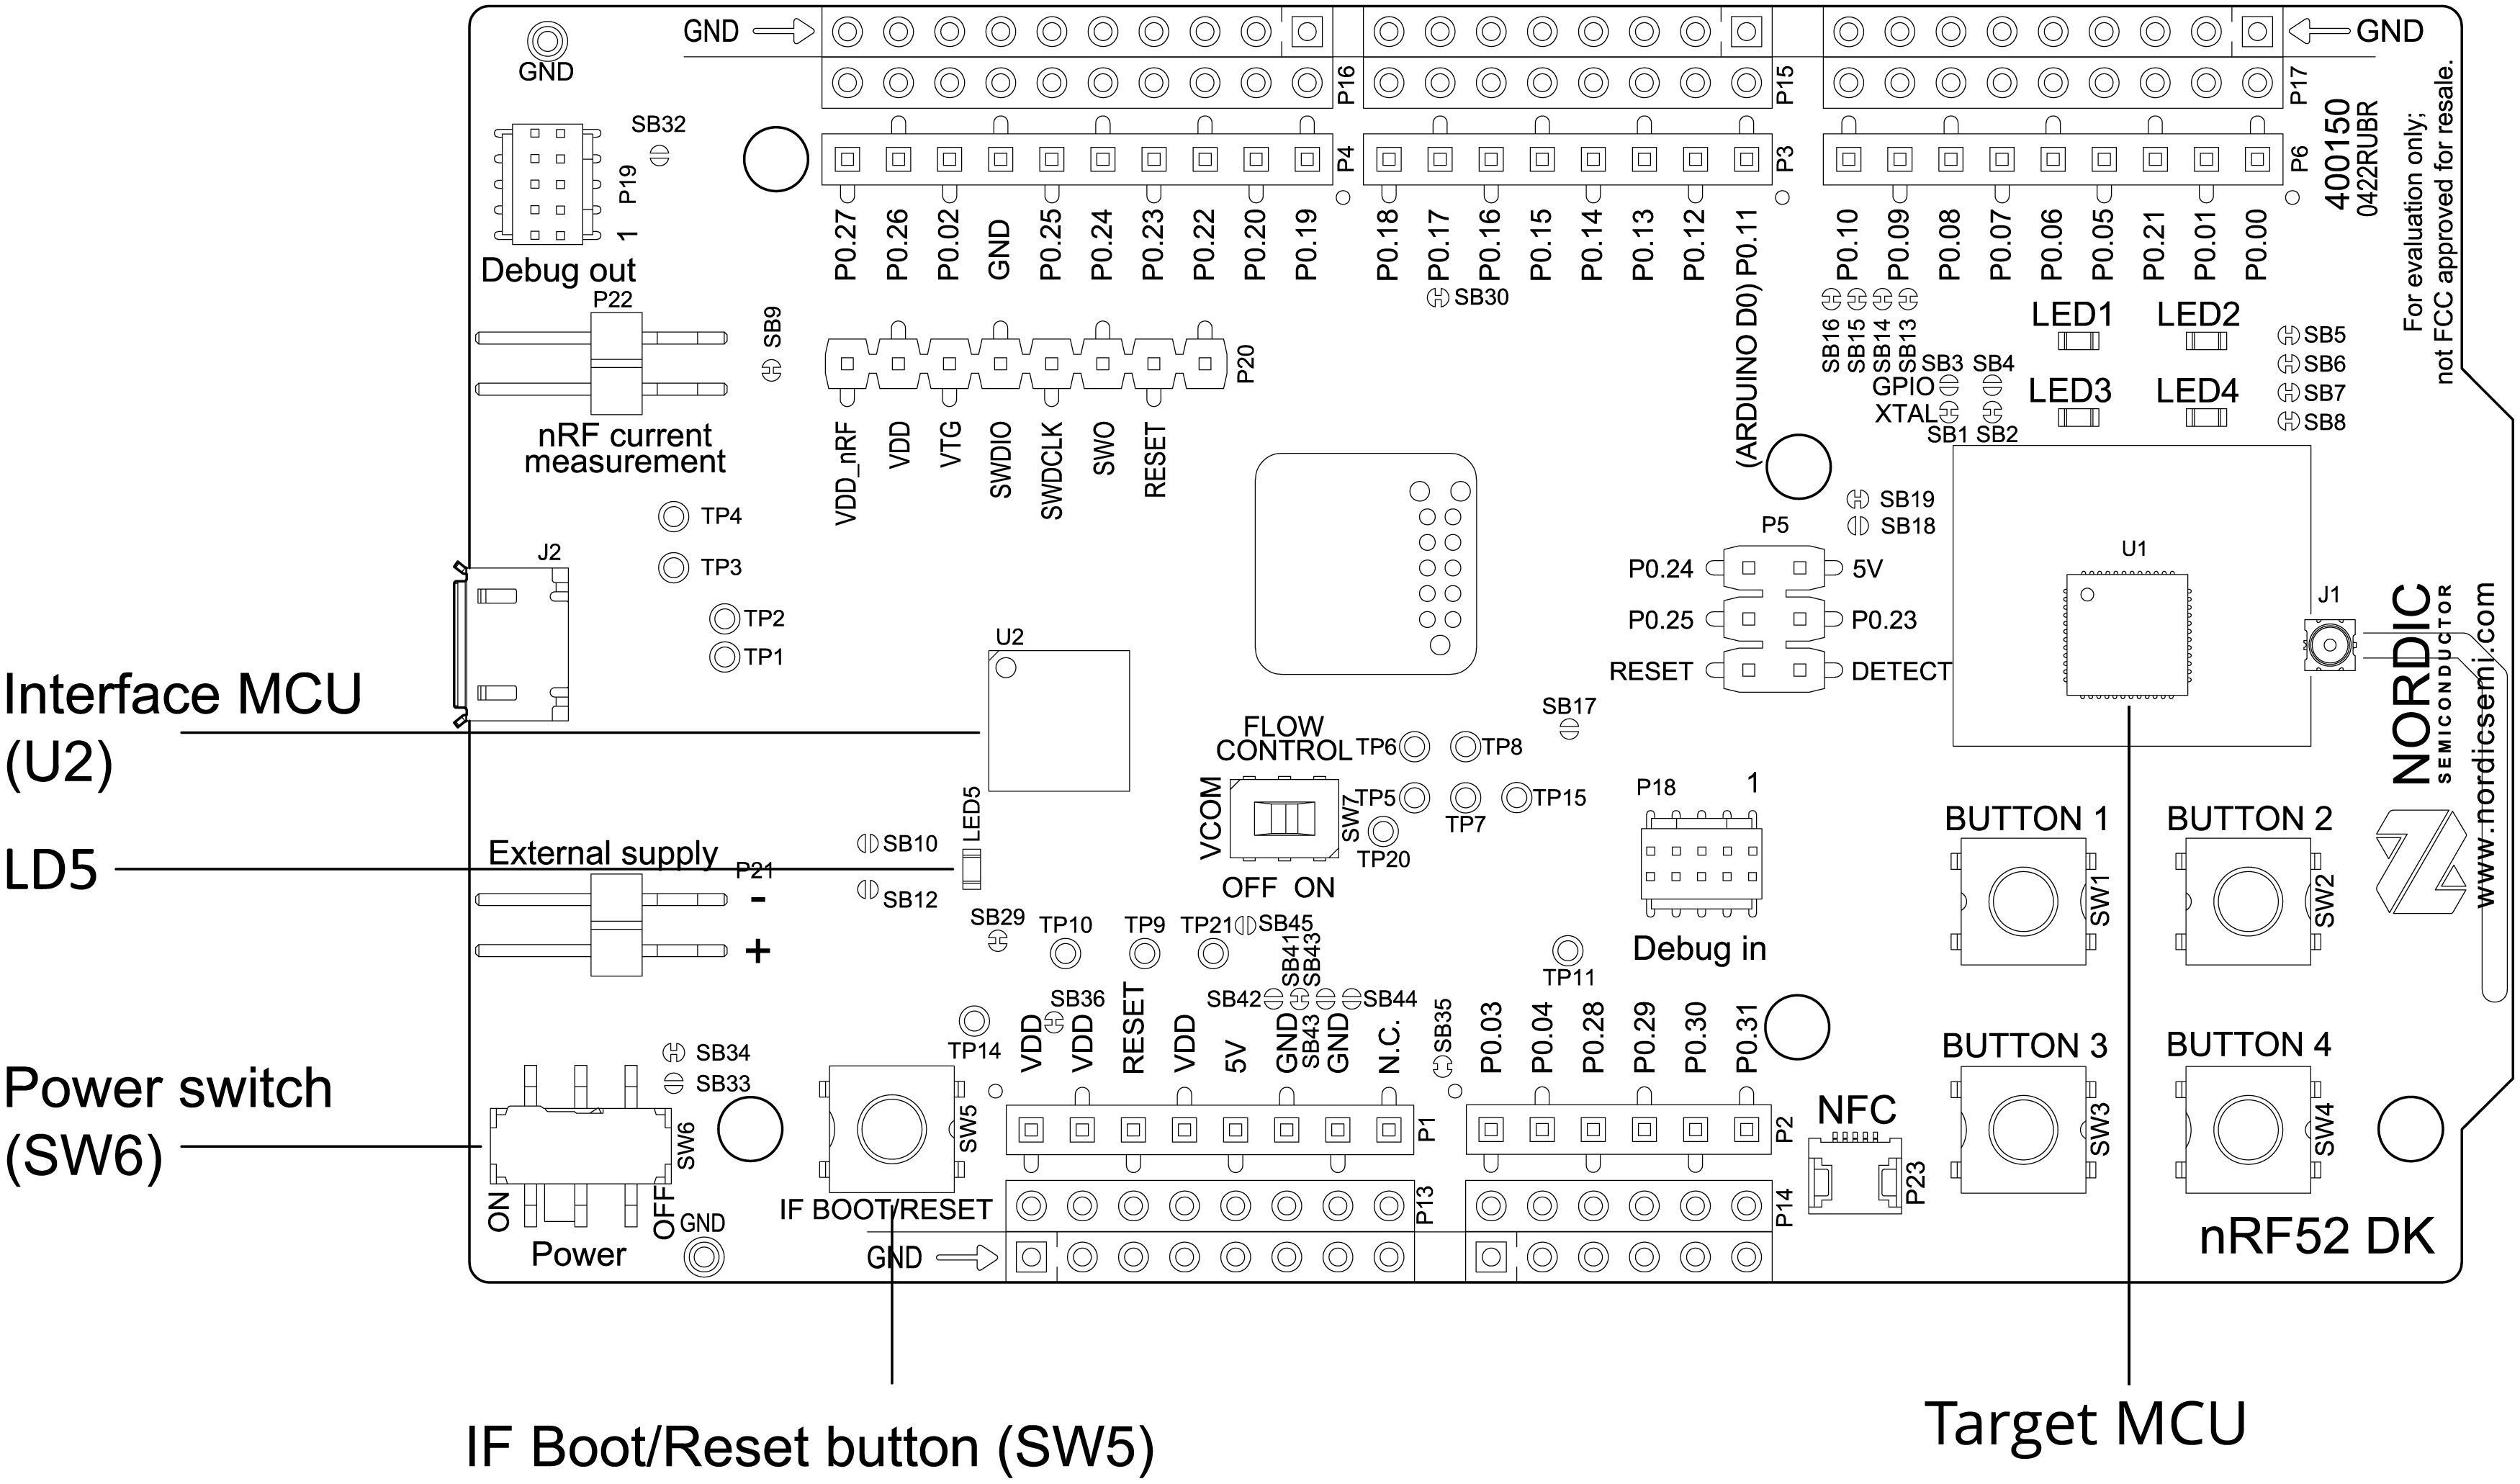
\includegraphics[width=.8\linewidth]{figures/pca10040_interface_mcu.png}
    \caption{Nordic nRF52 DK "Target" og "Interface" MCU}
    \label{fig:interface-mcu}
\end{figure}

\section{Praktisk rundt filene}

I denne laben får dere utlevert noen \verb|.c| og \verb|.h|-filer. Egne tabeller under hver oppgave lister opp alle filene som kommer med, samt litt informasjon om dere skal endre på filene eller om dere skal la dem forbli i løpet av oppgaven. Dere får også utdelt et utviklingsmiljø for feilsøking i VSCode. Utviklingsmiljøet er inkludert i hver oppgavemappe på Github. For mer info om utviklingsmiljøet se appendiks \ref{app:Debugging} og \verb|nrf52dk-environment| på \href{https://github.com/ITK-TTK4235/nrf52dk-environment}{Github}. 


\section{Introduksjon - Praktisk rundt laben}


I denne laben brukes ARM GCC som verktøykjeden for programmering av mikrokontrolleren. Denne typen verktøykjede kalles åpen kilde (open-source), og er en del av GNU-prosjektet.

For å gjøre denne laben litt lettere blir det lagt til en \verb|Makefile| for hver oppgave. Denne vil bygge kildekoden, sette opp riktig minnefordeling på prosessoren, og deretter skrive koden til den. I tillegg blir det også utdelt en undermappe ved navn \verb|.buid_system|. Denne inneholder det som skal til for å få koden til å kjøre på utviklingskitet. 

Det er ikke meningen at innholdet i \verb|.build_system|-mappen skal endres, men om man vil forstå hvordan koden henger sammen med hva som fysisk skjer på mikrokontrolleren, er det bare å ta en titt.

I tillegg skal dere lære dere hvordan man leser datablad. Det å kunne lese datablad er veldig viktig dersom man har lyst til å jobbe med mikrokontrollere senere, men også til eksamen.

\subsection{Makefile}

I denne laben blir det gitt ut ferdige \verb|Makefiler|. Slik som i \verb|Makefile|-øvingen, kaller man \verb|make| fra et terminalvindu i samme mappen som \verb|Makefilen| for å kompilere \verb|C|-koden. Dette vil genere en \verb|.hex|-fil som mikrokontrolleren kan kjøre i \verb|build|-mappen. I tillegg til \verb|make|, har denne \verb|Makefilen| også fem andre mål; \verb|make debug| vil kompilere \verb|C|-koden med debug-flagg for feilsøking av programmet, \verb|make erase| vil slette minnet til mikrokontrolleren, \verb|make recover| vil slette minnet til mikrokontrolleren og deaktiverer tilbakelesningsbeskyttelsen ("read-back") hvis den er aktivert, mens \verb|make clean| vil slette ferdigkompilert kode og \verb|hex|-filen fra datamaskinen. For å faktisk overføre \verb|hex|-filen over i programminnet til mikrokontrolleren bruker vi målet \verb|make flash|. {\bf{VIKTIG!:}} Første gangen man programmerer et nytt utviklingskit må man bruke \verb|make recover| og deretter \verb|make flash|. Dette er fordi mikrokontrolleren kommer forhåndsprogrammert med et skriverbeskyttet program. {\bf{Uten dette steget vil ikke \verb|make flash| fungere.}}

\subsection{Programmeringstaktikk}

For å sette ønskede registre på nRF52832-en bruker vi et kjent triks fra \verb|C|-programmering. Dette innebærer at man lager \verb|struct|s, som dekker nøyaktig det minnet man ønsker å endre - for dermed å \textit{typecaste} en peker til starten av minnet inn i \verb|struct|-en. Dette gjør det mulig å endre på det underliggende minnet ved å endre på \verb|struct|-ens medlemsvariabler.

Dette er definisjonen på \textit{memory mapped IO}; man gjør endringer som i software ser ut som vanlige lese- og skriveoperasjoner i samme minnerom som resten av programmet, men i bakgrunnen peker deler av dette minnet til registre hos perifere enheter. Dette er i kontrast til \textit{port mapped IO}, hvor egne instruksjoner brukes for å gjøre operasjoner i et disjunkt minneområde fra programmet (se forøvrig forelesningene for mer om dette tema).

\subsection{Datablad}


Tilpassede datasystemer er forskjellige fra vanlige datasystemer, fordi de er skreddersydde for en spesifikk oppgave. Ofte må de fungere med begrensede ressurser, og gjerne over lang tid kun drevet av et knappecelle-batteri. Derfor må man som oftest glemme en del generelle ting som gjelder uavhengig av plattform, og fokusere på ting som kun gjelder plattformen man arbeider på. Det er her datablad kommer inn.

Datablader er essensielt dersom man vil være god på å programmere tilpassede datasystemer. For nRF52 DK, gjelder \texttt{nRF52832 Product Specification} (denne finner dere i mappen \verb|datablad|). Det er viktig å bruke denne flittig, ettersom den gir en nokså kortfattet dokumentasjon som beskriver nøyaktig arkitekturen til datasystemet som blir brukt.

Det er lurt å sjekke ut appendiks \ref{app:datablad} for en kort innføring i hvordan man leser og bruker databladet i kontekst av memory mapped IO {\bf før} man begynner med oppgavene.




\subsection{Førstegangsoppsett av utviklingsmiljø}


Før man bruker nRF52 DK må man laste ned redskapene som trengs for å programmere den på Linux. Disse skal allerede være installert på PCene på Sanntidssalen. Dersom man ønsker å bruke en annen maskin må man installere avhengighetene beskrevet på \href{https://github.com/ITK-TTK4235/nrf52dk-environment}{Github}.



\subsection{Strategier for feilsøking}

Å feilsøke, også kalt å \verb|debugge|, mikrokontrollere kan være utfordrende på grunn av mangelen på interaktive verktøy og begrensede ressurser tilgjengelig på mikrokontrollere. Selv om kompilatoren luker ut de fleste feil, er man fremdeles utsatt for logiske feil. Det finnes imidlertid to vanlige metoder som kan brukes til å feilsøke program som kjører på tilpassede datasystemer som du kan lære om i denne laben. En av disse metodene er \verb|Seriell debugging| som innebærer å koble en seriell kabel, som oftest USB, (se oppgave \ref{sec:4-oppgave-UART}) mellom utviklingskitet og datamaskinen for å bruke et seriell terminalprogram for å skrive ut feilsøkingsdata (f.eks. \verb|sprintf|). Denne feilsøkingsstrategien er tilstrekkelig i de aller fleste tilfeller. 

Den andre metoden er å bruke et debuggingsprogram som kommuniserer med Interface MCU-en (se figur \ref{fig:interface-mcu}). Dette lar deg blant annet inspisere og endre på registre live og kan være svært nyttig for å debugge mikrokontrollere. Denne metoden blir beskrevet i appendiks \ref{app:Debugging} og anbefales på det sterkeste.


\end{alphasection}



\setcounter{section}{0}
